\section{Ergebnisse}
\subsection{Beobachtung mit den Teleskopen im Garten}
Hier konnte zunächst der Jupiter aufgrund seiner Helligkeit problemlos identifiziert werden. Es waren dabei drei Monde deutlich sichtbar (Abb!!!). \\
Der Orionnebel konnte durch Orientierung am Sternbild Orion ebenfalls schnell gefunden werden, allerdings war er aufgrund der geringen Öffnung des verwendeten Teleskops relativ lichtschwach und schwierig zu erkennen. \\
Der Mond war aus offensichtlichen Gründen problemlos zu erkennen. Es wurden hier ebenfalls einige Photos mit einer 35 mm-Spiegelreflexkamera (Canon) aufgenommen, die in (...) dargestellt sind. Diese Aufnahmen weisen allerdings eine durch das Seeing begrenzte Schärfe auf. Seeing bezeichnet die durch Turbulenzen in der Atmosphäre verursachte Unschärfe in Aufnahmen, welche sich nur mit großem Aufwand vermeiden lässt. \\
Auch $\eta$ Ori konnte mittels Starhopping gefunden werden.

\subsection{Beobachtung am 50 cm-Teleskop} 
Mit dem 50 cm-Teleskop wurde die 
\subsection{Freie Beobachtung mit dem 40 cm-Teleskop}
Es wurden hier verschiedene Objekte beobachtet, unter anderem: Jupiter, Mars, M51, M13, der Andromenda-Nebel und der Mond. \\
Bei Objekten wie Jupiter und Mars war die Auflösung insbesondere durch das Seeing begrenzt, sodass die Beobachtung nur mit beschränkter Qualität möglich war. Beim Mars trat der Effekt auf, dass der obere Teil eher rötlich und der untere Teil tendenziell blau erschien. Dies ist auf die unterschiedliche Brechung der verschiedenen Farben in der Erdatmosphäre zurückzuführen: Blaues Licht wird stärker gebrochen, sodass das blaue Licht für den Beobachter \enquote{weiter unten} ankommt als das rote. \\
Bei der Beobachtung von M 51, der schon beim Imaging beobachteten \enquote{Whirlpool-Galaxie}, konnten lediglich zwei, durch das Seeing bedingt verschwommene, Flecken wahrgenommen werden. \\
Bei M 13, einem Kugelsternhaufen, konnten dahingegen die Sterne gut unterschieden werden. \\
Der Andromenda-Nebel war bei sehr geringer Deklination (< 10 $^\circ$) nicht beobachtbar. \\
Bei der Beobachtung des Mondes fiel die sehr große Helligkeit auf. Weiter war insbesondere der plastische Eindruck der Mondkrater beindruckend. \\
Nachfolgend ist die Aufnahme des Jupiters mit seinen Monden dargestellt (ref{fig:jup}).
\begin{figure}[h!]
\centering
        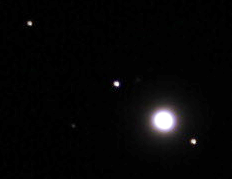
\includegraphics[width=.4\textwidth]{img_jup.png}
\caption{ Aufnahme des Jupiters mit drei sichtbaren Monden }
\label{fig:jup}
\end{figure}

Betrachtet man den Jupiter zum Zeitpunkt der Aufnahme (etwa 20:30 Uhr) in einem Astronomieprogramm (hier: Stellarium), so ergibt sich das in \ref{fig:scr} dargestelle Bild. 

\begin{figure}[h!]
\centering
        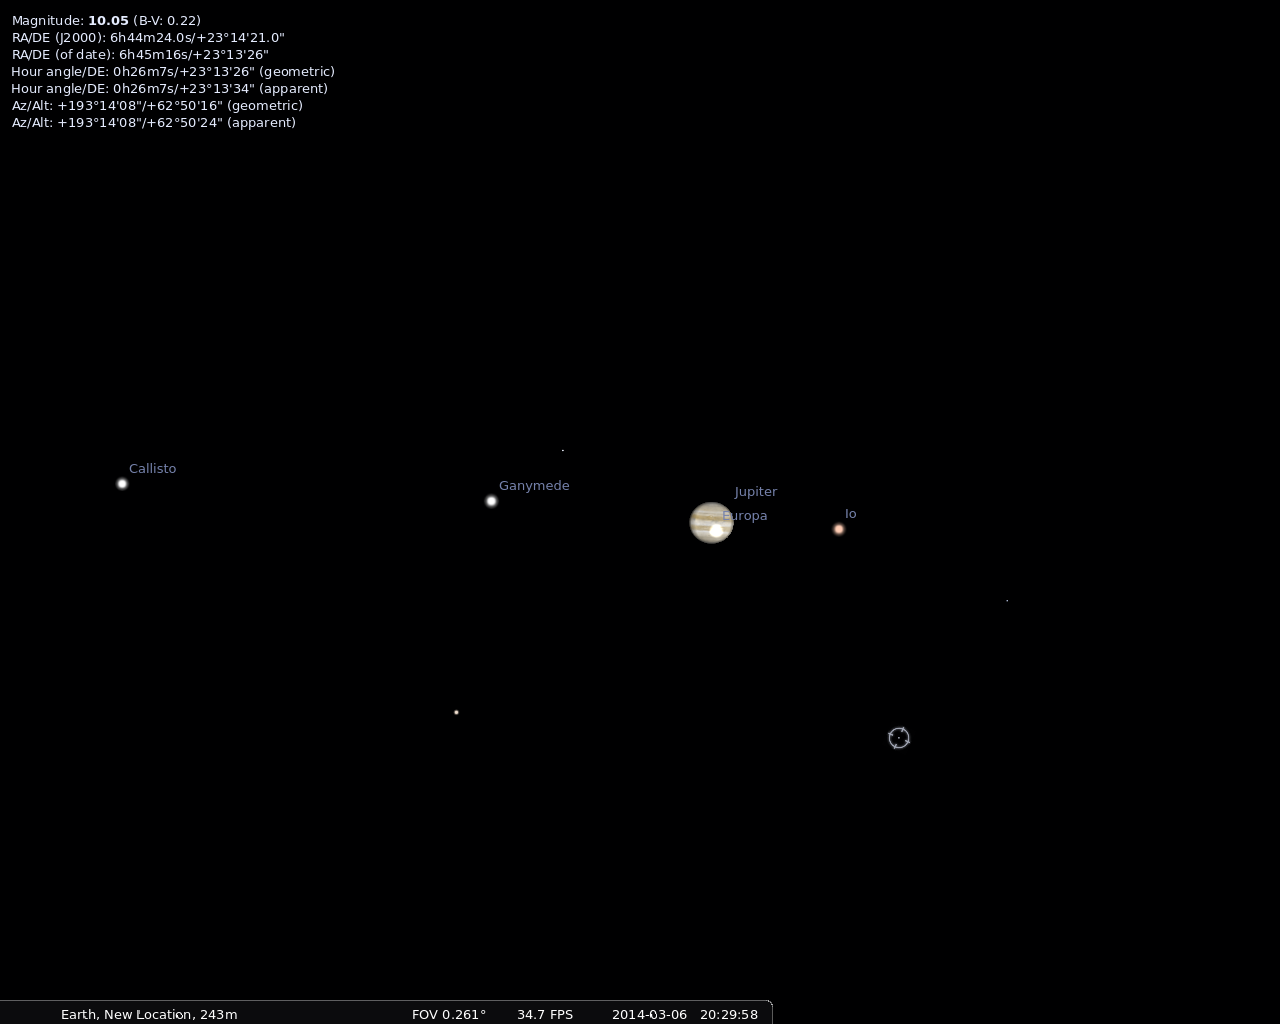
\includegraphics[width=.8\textwidth]{screenshot_jupiter2.png}
\caption{ Screenshot im Stellarium }
\label{fig:scr}
\end{figure}
Die in der Aufnahme sichtbaren Monde können somit von links nach rechts als Callisto, Ganymed und Io identifiziert werden. Europa befand sich zum Beobachtungszeitpunkt vor dem Jupiter, sodass dieser Mond nicht sichtbar ist. 